\chapter{绪论}

\section{研究背景及意义}

在应对大型复杂软件系统的设计与实现时,
越来越多的企业选择借鉴领域驱动设计中的思想与方法。
领域驱动设计(Domain-Driven Design, DDD)
是一种针对大型复杂软件系统的分析与建模方法,
由Eric Evans于2004年在其著作
《领域驱动设计:软件核心复杂性应对之道》\cite{DBLP:books/daglib/0013521}
中首次提出。
与传统的系统设计方式相比,领域驱动设计更加聚焦领域中的业务流程而非系统操作的数据,
强调领域模型的重要性。
% 领域模型中的每个领域对象都是高内聚的完整业务对象,可以直接进行复用;
领域驱动设计遵循关注点分离的原则,对领域对象进行了明确的策略和职责划分,
可以将现实业务映射到领域对象上,为领域专家与开发人员搭建沟通的桥梁。
通过领域驱动设计,开发团队和领域专家\cite{DBLP:books/daglib/0013521}深入交谈,
对业务了解更加准确,领域专家借助领域驱动设计的方法与开发团队进行沟通,
可以更好地对领域进行建模,并对建模的领域对象进行快速迭代修改,
同时将修改同步到实现层次上,
更加适应快速迭代的敏捷软件开发节奏。

领域驱动设计主要被分为战略建模(Strategic Modeling)
和战术建模(Tactical Modeling)两个层次\cite{millett2015patterns},
战略建模层次指导架构师及领域专家构架大型复杂软件系统并进行拆分,
战术建模层次指导开发者对拆分出的子系统进行落地。
战略建模层次的主要思想与方法十分契合当今流行的微服务架构(Microservice Architecture, MSA)\cite{nadareishvili2016microservice},且使用者多为经验丰富的架构师及领域专家,
所以战略建模能在高层次业务流程分析与系统划分时发挥作用;
战术建模层次则更加侧重于单个微服务或微服务中某一模块的落地,
并给出建模与实现过程中应该遵循的原则与约束。
战术建模是基于战略建模的结果,进行进一步抽象设计,
充当战略建模与最终技术实现的中间过渡阶段。
战术模式(Tactical Patterns)是战术建模中常用的表达业务问题的一种方式。
战术建模相比战略建模更加依赖领域模型(Domain Model)\cite{vernon2013implementing}
和通用语言(Ubiquitous Language)\cite{vernon2013implementing},
因为其需要通过战术模式将领域模型和通用语言中的概念映射到代码实现中,
代码实现也会随着领域模型的变化而重构,体现领域模型的改变。
战术建模还可以借助标准通用的战术模式,
让开发人员甚至非技术人员与架构师进行合作,参与到建模过程中来。

% 根据Vaughn Vernon的《实现领域驱动设计》\cite{vernon2013implementing}一书所述,
% 战术建模层次包括的重要概念有实体(Entity)、值对象(Value Object)、
% 领域服务(Domain Service)、领域事件(Domain Event)、聚合(Aggregate)等,
% 这些概念统称为战术建模模式。

上述领域驱动设计的两个层次都强调领域模型的重要性。
领域模型(Domain Model)是对领域中概念或对象的可视化表示,
专注于领域本身,可以用来分析业务,
发掘重要的业务领域概念,并建立业务领域概念之间的关系。
领域模型通常以从业务流程中分析提炼出的通用语言
为基础进行构建,并作为通用语言的核心。
通用语言(Ubiquitous Language)是将团队沟通与软件实现紧密联系到一起的一种基于模型的语言,
在应用通用语言进行领域建模时,领域专家和开发人员可以更好地
讨论需求、制定开发计划和描述系统特性。



% 使用模型驱动的方式来进行设计与实现,可以保障领域模型和具体实现代码的一致性,
% 并不断完善迭代领域模型,使其含义更加贴合业务流程,优化实现代码。

然而,领域驱动设计,特别是战术建模层次在领域建模实践时却面临许多挑战。
第一,战术建模中每种模式都是知识高度凝练的结果,包含了复杂的概念知识,
学习成本很高,没有大量的实践经验基本无法理解。
在建模实践时,难以准确把握各种模式的规范和约束,
无法正确地将战术建模模式与业务流程中的业务对象对应,
导致战术建模结果不标准、不统一,甚至战术建模结果错误,
难以发挥战术建模的优势;
第二,开发人员和架构师在使用战术建模时对业务的理解程度不同,
对模式的应用时机和实现技术看法不同,
导致架构师和开发人员无法在建模时进行顺畅地沟通,
不同开发人员的开发水平、经验也有差距,同一开发团队也往往很难让建模结果保持标准和统一;
第三,实施战术建模没有规范化的标准流程指导,
当前的一些建模工具(如Enterprise Architect\footnotemark[1]\footnotetext[1]{Enterprise Architect官网:https://sparxsystems.com}、
PlantUML \footnotemark[2]\footnotetext[2]{plantUML官网:https://plantuml.com})
对领域建模规则与约束的支持也不够完善,无法建立起足够通用的模型,
最终导致战术建模的结果无法规范化、标准化地应用。
上述挑战阻碍了开发者正确使用领域驱动设计战术建模。

% 导致战术建模难以实践的原因有很多。第一,战术建模这一概念本身就很复杂,
% 战术建模层次包含的概念知识十分丰富,且每一种模式都很复杂,
% 没有大量的实战经验基本无法理解,学习战术建模的成本很高;
% 第二,由于一线开发人员开发水平、经验差距较大,对领域驱动设计的理解也不够深入,
% 同一开发团队也往往很难让建模结果保持标准和统一;
% 第三,在实际应用战术建模时也没有工具支持规范化的流程和标准化的规则与约束,
% 当前的一些建模工具(如Enterprise Architect\footnote{Enterprise Architect官网:https://sparxsystems.com}、
% PlantUML \footnote{plantUML官网:https://plantuml.com})
% 对领域建模支持不够完善,对不熟悉战术建模的开发人员也没有指引与提示,
% 导致战术建模难以规范化、标准化地应用到实际建模设计当中。

为了解决上述挑战,本文提出了一种面向领域驱动设计的战术建模支持方法及工具,
具体工作内容如图\ref{workresult}所示。
战术建模方法包括一套标准化的\textbf{战术建模指南},
用于帮助理解不同模式的特征属性、
使用时机以及实现技术,作为领域建模的理论支撑指导建模过程;
根据战术建模指南,本文还基于UML的profile扩展机制实例化\textbf{战术建模语言},
用于规范化使用战术建模模式进行领域建模的流程;
基于所提出的战术建模方法,本文还实现了一种\textbf{战术建模支持工具},
支持可视化建模、验证建模结果以及存储和扩展建模结果,
为战术建模支持方法提供可视化方式展现。


\begin{figure}[h] %figure环境,h默认参数是可以浮动,不是固定在当前位置。如果要不浮动,你就可以使用大写float宏包的H参数,固定图片在当前位置,禁止浮动。
    \centering %使图片居中显示
    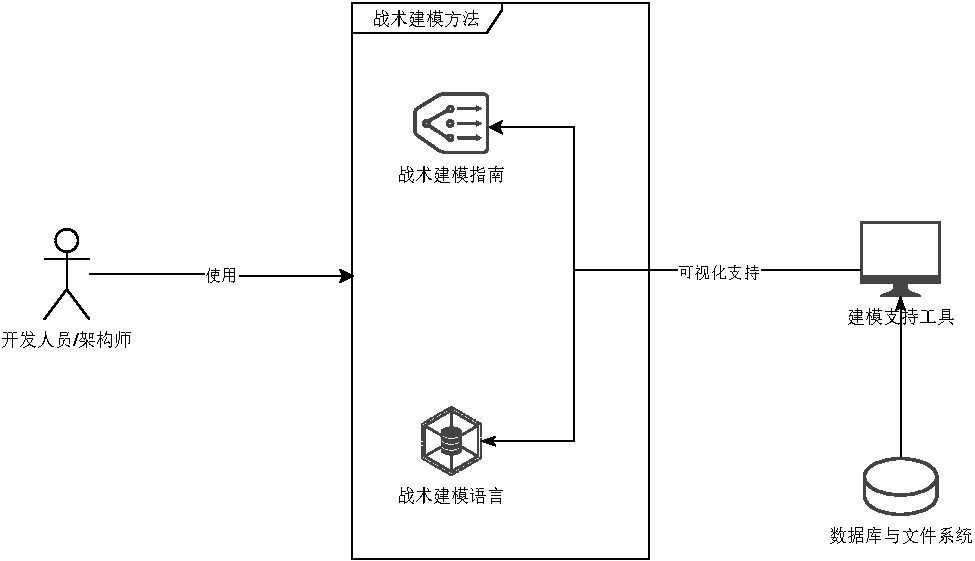
\includegraphics[width=0.8\textwidth]{FIGs/chapter1/workresult.pdf} %中括号中的参数是设置图片充满文档的大小,你也可以使用小数来缩小图片的尺寸。
    \caption{战术建方法及支持工具} %caption是用来给图片加上图题的
    \label{workresult} %这是添加标签,方便在文章中引用图片。
\end{figure}%figure环境



\section{国内外研究现状}


领域驱动设计自提出以来,受到了学术界与工业界的广泛关注。
战略建模层次的实践与实现代码关联不紧密,更多关注的是顶层设计与架构搭建,
实施者一般也拥有较多的开发经验与较高的建模水平,所以在国内外都能较好地进行落地。
但战术建模层次更加侧重于建模的设计过程和具体实现,
对于建模实施者的水平有较高的要求,
还需要通过统一标准化的流程来达到建模结果的准确性,
规范化的建模语言也是支持战术建模成功实施的必要条件。所以,
一套完整的战术建模支持方法及工具就显得格外重要。

特定领域建模语言(Domain Specific Modeling Language)\cite{{frank2013domain}}
是一种专注于某个特定领域,结合了特定领域知识和概念的建模语言。
可以使用特定领域建模语言来进行战术建模,
从而获得统一标准化且具有特定领域特征的建模结果。
目前国内外研究人员对特定领域建模语言的定义方法了一些研究。
Hao Wu等人\cite{wu2018workflow}指出,
可以通过UML结合对象约束语言(Object Constraint Language,OCL)
的方式来扩充医疗系统领域现有元模型,形成一种更为完整的建模语言及方法。
Kühlwein等人\cite{kuhlwein2019firmware}通过一种分层架构的思想来打通物联网领域的多种元模型,
构建了一种平台型的特定领域建模语言,其中每层都有针对不同设备的元模型,
通过该平台进行组织和交互,这种定义方法需要依赖较为成熟的元模型;
Jumagaliyev等人\cite{jumagaliyev2019modelling}通过对云存储平台的通用存储类型进行分析,
抽象出数据类型的特征属性,创建元模型并使用EuGENia\cite{kolovos2010epsilon}进行注释,
最终借助Eclipse IDE将创建的元模型转换为具体的图形建模框架编辑器,
不仅定义了特定于云存储平台的元模型,还提供了建模工具编辑器。

国内外研究人员也对领域驱动设计建模语言的定义进行了一些研究。
Florian Rademacher等人\cite{rademacher2017towards}根据领域驱动设计实践经验提出使用UML profile
定义元模型,并将其应用到微服务领域中去。
Florian Rademacher等人调研了大量领域建模的UML图,
确定了可以描述领域模型的UML类图的构造方法。通过扩展元类的方式,
达到了使用领域驱动设计战术建模实现微服务系统建模的目的,
并为验证模型有效性和实现微服务代码奠定了基础。
同样的,Hippchen等人\cite{hippchen2019systematic}也强调了微服务化拆分中应用面向领域驱动设计建模语言的好处。
Florian Rademacher等人强调了领域驱动设计概念在UML中缺少正式的定义,阻碍了模型的验证和转化,
但同时UML又符合软件设计领域建模的要求,应用也十分广泛,故以UML为基础进行扩展,
定义出了一套新的针对领域驱动设计相关规则和约束的建模语言。
Andreas Diepenbrock等人\cite{diepenbrock2017ontology}提出使用本体论(Ontology)\cite{smith2003ontology}
来定义针对微服务应用的领域驱动设计元模型,该研究主要使用了本体论在特定领域表达知识语义的功能,
结合领域驱动设计实现了建模的目的。

以上工作说明任何特定领域建模语言的定义与提出都需要前期大量领域实践知识的总结,
并且在已有工作成果的基础上进行元模型的定义效率更高。
由于领域驱动设计战术建模理论较为成熟,
目前定义的战术模式特征明确,所以,
本文将基于领域驱动设计战术建模的现有研究成果,
结合实际应用情况,进行修改和优化,
定义一套新的领域驱动设计战术建模语言。


除了定义元模型来实现建模语言之外,提供支持建模语言的工具也十分重要。
刘辉等人\cite{刘辉2008元建模技术研究进展}提出元建模工具的实现主要分为两种途径。
第一种是使用配置文件扩展通用建模工具,让通用建模工具支持特定领域的元模型从而支持特定领域建模语言。
Guerriero等人\cite{guerriero2018streamgen}通过UML的profile扩展机制,
扩展了现有UML的语法元模型,达到创建新的元模型的目的,
扩展UML语法元模型的实现方式只依赖于配置文档,有利于多种建模方法的集成,
但需要借助统一建模语言的实现平台,如MetaEdit+\footnotemark[3]\footnotetext[3]{MetaEdit+首页:https://www.metacase.com/products.html}。
第二种是通过建模工具生成器根据元模型直接生成相应的建模工具,
La Fosse等人\cite{la2019towards}使用GEMOC(一种基于Eclipse的特定领域语言创建平台)
来创建扩展元模型,生成了新的建模语言及支持工具,
这种方式定制化程度更高,可以提供独立的工具,
但生成的建模工具依赖工具生成平台,
如EMF(Eclipse Modeling Framework)\footnotemark[4]\footnotetext[4]{Eclipse Modeling Framework主页:https://www.eclipse.org/modeling/emf/}
提供的一系列生成元模型的工具。

许多国内外的研究人员对领域驱动设计建模语言的支持工具开展了实践与探究工作。
Duc Minh Le等人\cite{le2018domain}定义了一种名为DCSL的基于注释的特定领域建模语言,
通过注释约束了领域模型的特征与行为,由于Java语言对注释的良好支持,
采用Java开发了一款建模语言支持工具,摆脱了建模工具的平台依赖性,
但注释对模型的表达不够直观,仅仅依靠注释来表达建模过程和结果远远不够;
Kapferer等人\cite{kapferer2020domain}定义了一种战略建模语言,
并提供了相应的编辑、验证和转换工具,重点关注上下文映射工作,
实现支持工具借助了PlantUML建模平台,
达到了可视化建模支持。


虽然目前已有一些关于领域驱动设计建模的探索与研究,但仍然存在诸多问题。
首先,许多建模语言的提出以元模型为基础,但元模型的定义缺少理论依据,
导致元模型的定义不够规范化和标准化;
其次,建模语言的提出即使调研过大量文献,
也缺少对学术界与工业界实际应用差别的思考,
导致最终定义的建模语言脱离实际应用场景;
最后,战术建模的支持工具易用性不够,或者依赖太多额外平台,学习和使用成本过高,
导致难以应用到实际生产中去。
总的来说,战术建模流程缺少一套标准化的建模支持方法及工具。

\section{本文主要研究工作}

本文主要的研究工作分为以下三个方面:

1.围绕领域驱动设计的战术建模过程展开了理论调研,
从《领域驱动设计:软件核心复杂性应对之道》\cite{DBLP:books/daglib/0013521}和
《实现领域驱动设计》\cite{vernon2013implementing}两本著作中抽取了八种战术建模模式及其重要特征。
具体地,针对八种战术建模模式,
设计了调查问卷,与工业界具有领域驱动设计实战经验的架构师和开发人员展开访谈;
根据访谈结果,通过多次焦点小组讨论,
对八种战术建模模式及其重要特征进行验证和完善,
克服了理论脱离实际的问题。
最终得出一套战术建模指南,该指南包括战术建模模式、模式属性、使用时机以及实现技术。


2.基于上述理论基础,通过UML profile机制扩展UML元类,实例化战术建模语言。
战术建模语言描述了战术模式的构造型、必要属性、关联关系以及重要约束。
以UML中元类为基础,更符合软件设计中面向对象(Object-Oriented)的思想,
也更易于软件从业者接受和学习。以该元模型为基础的建模语言,更关注战术建模,
包含最贴合实践的规则和约束,建模效率更高。

3.实现了一个战术建模支持工具,
该工具对建模过程中使用的战术模式进行约束与规范性校验,
对建模结果进行多种格式的转化与存储,
还包含生成框架项目代码包等扩展功能。
对战术建模支持工具进行了功能测试,并使用该工具进行了战术建模案例研究,
结果表明该工具支持开发人员快速理解各种战术模式的重要特征和规则约束,
降低了使用战术建模的学习成本;
可以对建模结果进行验证并提示开发人员进行修改,规范化建模过程;
还具有将建模结果转化为多种格式文件和框架项目代码的功能,使建模结果更具有通用性。


上述战术建模指南、战术建模语言以及战术建模支持工具共同组成了本文研究工作的战术建模支持方法及工具。

\section{本文组织结构}

本文组织结构如下:

第一章~绪论。介绍了本文的研究背景、国内外研究现状以及本文主要的研究工作;

第二章~理论与技术支持。介绍领域驱动设计尤其是战术建模设计相关理论和概念,对建模语言原理以及支持工具实现方法进行介绍;

第三章~面向领域驱动设计的战术建模支持方法。通过文献综述、访谈和焦点小组提出战术建模支持方法,
并详细介绍了该战术建模支持方法;

第四章~建模支持工具设计与实现。介绍本文如何基于第三章得到的战术建模方法实现一个建模支持工具,
介绍对该工具的需求分析,工具整体架构与各模块的设计和实现;

第五章~建模支持工具测试与案例研究。对建模支持工具进行功能测试、性能测试和案例分析研究,
介绍了使用建模支持工具建模的流程和效果;

第六章~总结与展望。总结本文所做的研究工作和贡献,分析工作不足之处,并对后续研究进行了展望。
